% Template for a Thesis
%
% 3-tokenization.tex
%
% Tokenization

\chapter{Tokenization}\label{sec:tokenization}

\section{Introduction}

Tokenization is the first major step in language processing. Once the corpus is obtained, before starting to process the text, because we're dealing with language, we want to understand the meaning of the text. \textbf{Tokens} in the language have a semantic meaning, be it words, phrases, symbols or other elements, whereby a meaning is assigned to each token. Tokenization is the process of breaking a stream of text up into tokens.~\cite{manning2008introduction}

The way to tokenize heavily depends on the task afterwards. Some applications might require different tokenization algorithms. Nowadays, most deep learning architectures in NLP process the raw text at the token level and as a first step, create embeddings for these tokens, which will be explained in more detail in the following sections.~\ref{subsec:wordemb} In short, the type of tokenization depends on the type of embedding. There are several, explained further in the following sections, and each has its advantages and drawbacks.~\ref{subsec:toktypes}

\paragraph{What is a token?}

A token is an instance of a sequence of characters in some particular document that are grouped together as a useful semantic unit for processing. Here is an example of tokenization.

\begin{quote}
    Input: I ate a burger today, and it was good.\\
    Output: ['I', 'ate', 'a', 'burger', 'today', 'and', 'it', 'was', 'good']
\end{quote}

In this example, the way to obtain tokens looks simple: just locate word boundaries, split by whitespace and get the symbols, and remove the punctuation marks, since punctuation marks have no definite meaning. However, this is not always the case.

\paragraph{How to deal with punctuation marks?}

Each language has its own set of tricky cases, for example in English what is the correct approach when dealing with apostrophes for possession and contractions? For example words like \emph{aren't}, \emph{Sarah's} and \emph{O'Neill}. Because of this, it is imperative to know the language of the text to be tokenized. \textit{Language identification} is the task of identifying the language of the input text. From the initial k-gram algorithms used in cryptography (Konnheim, 1981), to more modern n-gram methods (Dunning, 1994) have been used. Once the language is known, we can follow the rules for each case and deal with punctuation marks appropriately.

\paragraph{Other types of tokens}

Additionaly, tokens can be either characters or \textbf{subwords}. For example, the word \emph{smarter}:

\begin{quote}
    Sentence: the smarter computer
    Word: the, smarter, computer\\
    Word without word boundaries: the smart, er comput, er\\
    Character tokens: t-h-e, s-m-a-r-t-e-r, c-o-m-p-u-t-e-r\\
    Subword tokens: the, smart-er, comput-er
\end{quote}

The major question in the tokenization phase is: \textit{what are the correct tokens to use?}. The following section explores these 4 types of tokenization methods and delves into the algorithms and code libraries available.

\section{Tokenization algorithm types}\label{subsec:toktypes}

\subsection{Word level tokenization}

Word level tokenization was the first tokenization type used, and is also the most common. It splits a piece of text into individual words based on word bounderies, usually a specific delimiter, mostly whitespace ' ' or other punctuation signs.

Conceptually, splitting on whitespace can also split an element which should be regarded as a single token, for example New York. This is mostly the case with names, borrowed foreign phrases, and compounds that are sometimes written as multiple words. Word level tokenization without word boundaries aims to address that problem.~\ref{subsec:wordtokwowb} on page~\pageref{subsec:wordtokwowb}

\subsubsection{Word level algorithms}

The most simple way to obtain word level tokenization is by simply splitting the sentence on the desired delimeter, whitespace usually. The \pyth{sentence.split()} function in Python or a Regex command \pyth{re.findall("[\w']+", text)} achieve this in a simple way.

The \href{https://www.nltk.org/}{natural language toolkit (NLTK)} in python provides a \href{https://www.nltk.org/api/nltk.tokenize.html}{tokenize package} which includes a \emph{word\_tokenize} function, which requires the user to give in the language of the text. If none is given, English is taken as default.

\begin{python}
from nltk.tokenize import word_tokenize
sentence = u'I spent $2 yesterday'
sentence_tokenized = word_tokenize(sentence, language='English')
>>> sentence_tokenized = ['I', 'spent', '$', '2', 'yesterday']
\end{python}

Similarly, SpaCy offers a similar functionality. It is possible to load the language model for a different language and model size.

\begin{python}
import spacy
sp = spacy.load('en_core_web_sm')
sentence = u'I spent $2 yesterday'
sentence_tokenized = sp(sentence)
>>> sentence_tokenized = ['I', 'spent', '$', '2', 'yesterday']
\end{python}

Keras also offers a similar functionality:

\begin{python}
from keras.preprocessing.text import text_to_word_sequence
sentence_tokenized = text_to_word_sequence(sentence)
\end{python}

As does Gensim:

\begin{python}
from gensim.utils import tokenize
sentence_tokenized = list(tokenize(sentence))
\end{python}

\paragraph{Word embeddings}\label{subsec:wordemb}

As stated before, the goal of tokenization is to split the text into units with meaning. Typically, each token is assigned an embedding vector: Mikolov et al., 2013~\cite{mikolov2013efficient} introduced word2vec, as a way of transforming a word into a fixed-size vector representation, as shown in the picture below.

\begin{center}
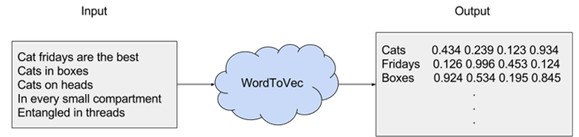
\includegraphics[width=12cm]{figures/word_emb.png}
\end{center}

If viewed abstractly in its N dimensions, each word's representation is close to similar words. As a simple example:

\begin{quote}
    Word: smart, embedding: [2, 3, 1, 4]\\
    Word: intelligent, embedding: [2, 3, 2, 3]\\
    Word: stupid, embedding: [-2, -4, -1, -3]
\end{quote}

The embedding numbers are just as an example, to illustrate the distances between words. For example, \emph{smart} and \emph{intelligent} have a distance of 2, since the last 2 numbers in the vector differ by one respectively. If this was plotted in a 4 dimensional space, these words would be very close together. On the other hand, \emph{stupid} is almost the opposite of \emph{smart}. The distance in this case is much higher. In the plot, these words would be very far apart.

As well as word2vec, there are other word embedding algorithms such as GloVe or fasttext.

Thus, with word embeddings, a sentence is transformed into a sequence of embedding vectors, which is very useful for NLP tasks.

\subsubsection{Word level drawbacks}

Word embeddings have some drawbacks however. In many cases, a word can have more than one meaning: \emph{well}, for example, can be used in these 2 scenarios.

\begin{quote}
    I'm doing quite well.\\
    The well was full of water.
\end{quote}

In the first case, well is an adverb while in the second it's a noun. \emph{well}'s embedding will probably be a mixture of the two, since word embeddings don't generalize to homonyms.

Another drawback is that word embeddings aren't well equipped to deal with out of vocabulary (oov) words. Word embeddings are created with a certain vocabulary size, that is, a certain number of words are known. If afterwards a new word arrives which isn't present in the vocabulary, because it's a foreign word, or a misspelled word, it will be given an unknown <UNK> embedding, that will be the same for all unknown words. Therefore all unknown words have the same embedding, that is, the NLP task will treat all these words as if they had the same meaning. The information within these words is lost due to the mapping from OOV to UNK.

Another issue with word tokens is related to the vocabulary size. Generally, pre-trained models are trained on a large volume of the text corpus. As such, if the vocabulary is built with all the unique words in such a large corpus, it creates a huge vocabulary. This opens the door to \emph{character tokenization}, since in this case the vocabulary depends on the number of characters, which is significantly lower than the number of all different words.

These problems are not to be mistaken with tokenization problems, tokenization is merely a way to an ends, they're mostly used to create embeddings. And if embeddings from word tokens are problematic, the tokenization method is changed in order to create different tokens, in order to create other types of embeddings.
    
\subsection{Character level tokenization}

In this type of tokenization, instead of splitting a text into words, the splitting is done into characters, whereby \emph{smarter} becomes \emph{s-m-a-r-t-e-r} for instance. \href{https://github.com/karpathy/char-rnn}{Karpathy, 2015} was the first to introduce a character level language model.

OOV words, misspellings or rare words, are handled better, since they're broken down into characters and these characters are usually known. In addition, the size of the vocabulary is significantly lower, namely 26 in the simple case where only the English characters are considered, though one might as well include all ASCII characters. Zhang et al., 2015~\cite{zhang2015text}, who introduced the character CNN, consider all the alphanumeric character, in addition to puctuation marks and some special symbols.

Character level models are unrestricted in their vocabulary and see the input "as-is". Since the vocabulary is much lower, the model's performance is much better than in the word tokens case. Tokenizing sequences at the character level has shown some impressive results, as stated below.

Radfor et al., 2017~\cite{radford2017learning} from OpenAI showed that character level models can capture the semantic properties of text.

Kalchbrenner et al., 2016~\cite{kalchbrenner2016neural} from Deepmind and Leet et al., 2017~\cite{lee-etal-2017-fully} both demonstrated translation at the character level. These are particularly compelling results as the task of translation captures the semantic understanding of the underlying text. Spelling mistakes, rare words and morphological aspects are very well handled with this type of tokenization.

\subsubsection{Character level algorithms}

The previous libraries explored in the case of word embeddings (native python libraries, nltk, spacy, keras) have their own version for character level tokenization.

\subsubsection{Character level drawbacks}

When tokenizing a text at the character level, the sequences are longer, which takes longer to compute since the neural net needs to have significantly more parameters to allow the model to perform the conceptual grouping internally, instead of being handed the groups upfront.

In addition, it becomes challenging to learn the relationship between the characters to form meaningful words. Besides, there is no semantic information among characters, characters are semantically void.

Sometimes the NLP task doesn't need processing at the character level, such as when doing a sequence tagging task or name entity recognition, the character level model will output characters, which requires post processing.

As an in-betweener between word and character tokenization, subword tokenization produces subword units, smaller than words but bigger than just characters.

\subsection{Subword level tokenization}

Subword tokenization is the task of splitting the text into subwords or n-gram characters. For example, words like lower can be segmented as low-er, smartest as smart-est, and so on. In the event of an OOV word such as \emph{eorner}, this tokenizer will divide it into \emph{eorn, er} and effectivey obtain some semantic information. Very common subwords such as \emph{ing}, \emph{ion}, usually with a morphological sense, are learnt through repetition. The word \emph{unfriendly} would be split into \emph{un, friend, ly}.

Nowadays, as of 2020, the most powerful deep learning architectures are based on Transformers, introduced by Vaswani et al., 2017~\cite{vaswani2017attention} and these rely on subword tokenization algorithms to prepare the vocabulary.

\subsubsection{Subword level algorithms}

Since Transformers are a relatively architecture at the time of writing, subword tokenization is an active area of research. Nowadays three algorithms stand out: byte-pair encoding (BPE), unigram LM, WordPiece and SentencePiece.

Since BPE is the basis of the thesis, it will be explained in depth in the following section. The rest of the algorithms follow below.

Huggingface, a popular NLP framework, released Transformers and Tokenizers in 2019 by Wolf et al.,~\cite{wolf2019huggingfaces}. They include \href{https://github.com/huggingface/tokenizers/tree/74d812d40180032d2dbb6ca59e2e10f0257ef46b/bindings/python/tokenizers/implementations}{several subword tokenizers} such as \emph{ByteLevelBPETokenizer}, \emph{CharBPETokenizer}, \emph{SentencePieceBPETokenizer} and \emph{BertWordPieceTokenizer}. The first refer to the first subword level algorithm, BPE, in addition to WordPiece and Sentencepiece.

\paragraph{Unigram LM}

Unigram language modeling was introduced by Kubo, 2018~\cite{kudo-2018-subword}. It's based on the assumption that all subword occurrences are independent and subword sequences are produced by the product of subword occurrence probabilities. Both WordPiece and Unigram Language Model leverages languages model to build subword vocabulary. This is the rough pipeline of the algorithm:

\begin{enumerate}
    \item Prepare a large enough corpus.
    \item Define a desired subword vocabulary size.
    \item Optimize the probability of word occurrence by giving a word sequence.
    \item Compute the loss of each subword.
    \item Sort the symbol by loss and keep top X \% of word (e.g. X can be 80). To avoid out-of-vocabulary, character level is recommend to be \item included as subset of subword.
    \item Repeating step 3–5until reaching subword vocabulary size which is defined in step 2 or no change in step 5.
\end{enumerate}

The author argues that BPE is based on a greedy and deterministic symbol replacement, which can't provide multiple segmentations with probabilities. The unigram LM model is more flexible than BPE because it's based on a probabilistic LM and can output multiple segmentations with their probabilities.

\paragraph{WordPiece}

https://medium.com/@makcedward/how-subword-helps-on-your-nlp-model-83dd1b836f46
https://stackoverflow.com/a/55416944/4569908
% original tokens = ["John", "Johanson", "'s",  "house"]
% bert_tokens == ["[CLS]", "john", "johan", "##son", "'", "s", "house", "[SEP]"]

Byte Pair Encoding falter outs on rare tokens as it merges the token combination with maximum frequency.

WordPiece Tokenization is almost similar to Byte Pair Encoding. The only difference lies in the way we merge up the tokens to produce new tokens. While in BPE, we use the max frequency of the new token for merging but in WordPiece, we also take in consideration the frequency of two tokens separately used for merging apart from the frequency of the new token. This means if we have 2 token A \& B, we will be calculated:

Score(A,B) = Frequency(A,B)/Frequency(A)*Frequency(B) and max value pair will be selected

This definitely has an edge over Byte Pair Encoding.

It might be the case that Frequency(‘so’,’ on’) is very high but their separate frequencies are also high, hence if using WordPiece , we won’t be merging ‘soon’ as the overall score might go low. Again if Frequency(‘Jag’,’gery’) might be low but if their separate frequencies are also low, we will merge to form ‘jaggery’.

4. Unigram Language Model:

Let’s see the below example:

Even if we merged ‘face’+’d’ over ‘no’+’d’, it doesn’t mean we won’t encounter ‘nod’ ever. It just means that the probability of ‘nod’ is lesser but not 0. But if we use WordPiece, we might miss this.

So, what do to now?

What we need is a model that provides us with the probability of different tokens that can be generated. This simply means if we get the word ‘nod’, we shall get probabilities for ‘no+d’, ‘n+od’,’ nod’ but with different probabilities given the case these tokens (no,d, n, od, nod) are given in the initial vocabulary.

Let’s explore the Unigram Language model now

Read more in https://medium.com/data-science-in-your-pocket/tokenization-algorithms-in-natural-language-processing-nlp-1fceab8454af

\paragraph{SentencePiece}

https://github.com/google/sentencepiece

Sentencepiece is a less common, but very beautiful strategy for subword tokenization. While conceptually similar to BPE, it strays from the eager encoding strategy to allow it to achieve higher quality tokenization and reduce error induced by location-dependence seen in BPE. The main difference is how Sentencepiece views ambiguity in character grouping, seeing it as a source of regularization for downstream models during training, as well as its use of a simple language model to evaluate the most likely character groupings instead of eagerly picking the longest recognized string like BPE does. This results in very high quality tokenization, but comes at great cost to performance, at times making it the slowest part of an NLP pipeline. While the assumption of ambiguity in tokenization seems natural, it appears the performance trade-off is not worth it, as Google itself opted not to use this strategy in their BERT language model.

https://www.thoughtvector.io/blog/subword-tokenization/
https://www.thoughtvector.io/blog/subword-tokenization/Sentencepiece.svg

https://medium.com/@makcedward/how-subword-helps-on-your-nlp-model-83dd1b836f46

See medium link from wordpiece section

% https://www.quora.com/NLP-What-does-it-mean-Tokenizing
% https://www.quora.com/Why-is-tokenization-important-in-NLP
% https://en.wikipedia.org/wiki/Lexical\_analysis#Tokenization

\subsubsection{Subword level drawbacks}

\subsection{Tokenization without word boundaries}\label{subsec:wordtokwowb}

Another type of tokenization, beyond word, character or subword, is tokenization without subword boundaries. The three types of tokenization explored until now cannot create units among words, that is, they consider words separatedly.

Word and character level tokenization are deterministic, meaning that for a given word, its tokenization will always be the same. But in subword tokenization, a word like \emph{imagination} might have different tokenization, for example: \emph{im, agina, tion}, \emph{imagina, tion}, etc. It depends on the corpus that the subword tokenization algorithm is trained on, but there is no foolproff and/or unique tokenization.

Besides, when dealing with languages that don't include space tokenization, such as several Asian languages, an individual symbol can resemble a syllable rather than a word or letter. Additionally, most words are short (the most common length is 2 characters), and given the lack of standardization of word breaking in the writing system or lack of punctuation in certain languages, it is not always clear where word boundaries should be placed.

An approach to handle this has been to abandon word-based indexing, and do all indexing from just short subsequences of characters (character -grams), regardless of whether particular sequences cross word boundaries or not. Hence, at times, each character used is taken as a token in Chinese tokenization.

\section{BPE}

Byte Pair Encoding (BPE), first introduced by Sennrich et al., 2015~\cite{sennrich2015neural}, is a widely used tokenization method among Transformer-based models. It's a word segmentation algorithm that merges the most frequently occurring character or character sequences iteratively. Here is an example of a sequence in its original form and after the BPE merges, much shorter than the original.

\begin{center}
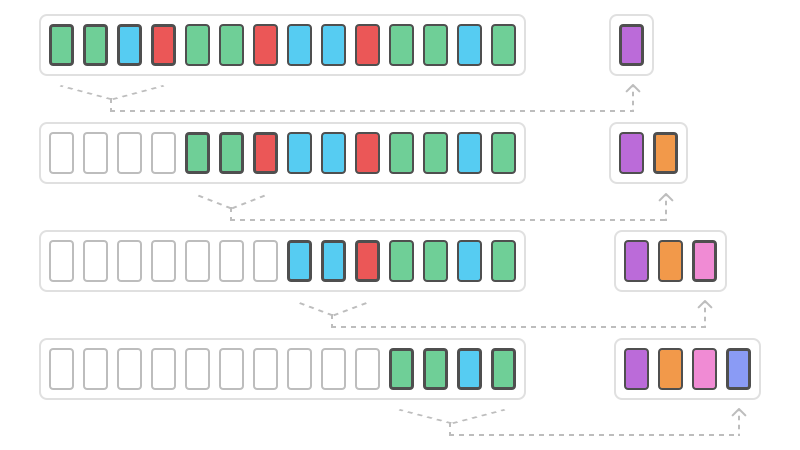
\includegraphics[width=12cm]{figures/bpe.jpg}
\end{center}

BPE enables the encoding of rare words with appropriate subword tokenization without introducing any 'unknown' tokens.

BPE addresses the issues of word and character tokenizers in the following ways: regarding OOV words, BPE segments OOV as subwords and represents the word in terms of these subwords. Regarding the longer sequence length which was one of the drawbacks of character tokenization, in this case the length of input and output sentences after BPE are shorter compared to character tokenization.

\subsection{Minimal algorithm to learn BPE segmentations}

These are the steps to learn BPE segmentations:

\begin{enumerate}
    \item Split the words in the corpus into characters after appending </w>, or another special symbol to show the beginning or end of the word.
    \item Compute the frequency of each pair of characters or character sequences in corpus and obtain the most frequent one.
    \item Save the best pair to the vocabulary.
    \item Merge the most frequent pair in corpus.
    \item Repeat steps 3 to 5 for a certain number of iterations.
\end{enumerate}

As an example, let's consider a simple corpus with a single line, and the character \emph{'\_'} to mark the beginning of each word, so as not to merge anything between different words later. The following code shows the first step of the algorithm.

\begin{python}
def read_corpus(corpus):
    tokens = [("_" + " ".join(token)) for token in corpus]
    return tokens

corpus = ['this is this.']
tokens = read_corpus(corpus)
>>> tokens = ['_t h i s _i s _t h i s .']
\end{python}

After that, we can initialize the vocabulary, which for now consists solely of the unique characters in the corpus. The following code snippet shows the second and third step.

\begin{python}
from collections import Counter

def get_stats(tokens):
    pairs = Counter()
    for sent in tokens:
        for word in sent[1:].split(' _'):
            symbols = ('_' + word).split()
            for j in range(len(symbols) - 1):
                pairs[symbols[j], symbols[j+1]] += 1
    return pairs

merge_list = []
pairs = get_stats(tokens)
>>> pairs = Counter({('_t', 'h'): 2, ('h', 'i'): 2, ('i', 's'): 2, 
                    ('_i', 's'): 1, ('i', 's,'): 1, ('_', 'i'): 1, 
                    ('_i', 't'): 1, ('t', '?'): 1})

most_frequent = pairs.most_common(1)[0][0]
merge_list.append(most_frequent)
>>> most_frequent = ('_t', 'h')
\end{python}

There we can see each bigram and its frequency. For example, ('\_t', 'h') occurs twice in the corpus, and it is taken as the most frequently occurring bigram, which we can save into the merge\_list. Now it's the time to merge this pair in the corpus.

\begin{python}
import re

def merge_pair_in_corpus(tokens, pair):
    # convert list of sentences into one big string 
    # in order to do the substitution once
    tokens = '\n'.join(tokens)
    # regex to capture the pair
    p = re.compile(r'(?<!\S)' + re.escape(' '.join(pair)) + r'(?!\S)')
    # substitute the unmerged pair by the merged pair
    tokens = p.sub(''.join(pair), tokens)
    tokens = tokens.split('\n')
    return tokens

tokens = merge_pair_in_corpus(tokens, most_frequent)
>>> tokens = ['_th i s _i s _th i s .']
\end{python}

Now the only thing left to do is to iterate this a number of times, which is usually decided by the user, until a certain number of pairs have been found. At each step, the object \emph{pairs} is calculated again since there might be new pairs such as ('\_th', 'i') in this example. The whole minimal code would look like this:

\begin{python}
corpus = ['this is this.']
merge_list = []
num_merges = 10

tokens = read_corpus(corpus)

for _ in range(num_merges):

    pairs = get_stats(tokens)
    most_frequent = pairs.most_common(1)[0][0]
    merge_list.append(most_frequent)
    tokens = merge_pair_in_corpus(tokens, most_frequent)
\end{python}

In each step of the iteration, the \emph{get\_stats} function iterates all the characters in the corpus, so the complexity is O(len(corpus) * len(sent)), for an average sentence length. Obtaining the most frequent pair takes constant time, since the object \emph{pairs} is a Counter object and has a built-in function to retrieve the most frequent item. At the step of \emph{merge\_pair\_in\_corpus}, the corpus is iterated in its entirety again, with a complexity of O(len(corpus) * len(sent)). Therefore, the algorithm has a complexity of O(num\_merges * len(corpus) * len(sent)). The num\_merges part cannot be avoided, but operating through all the characters of the corpus is very computationally expensive. In this thesis this algorithm has been optimized, as will be shown below.

\subsection{Applying BPE to OOV words}

In the event of an OOV word, such as \emph{these}, which the corpus used in the previous example doesn't know, the BPE algorithm can create some subword units from the corpus used before. This is Sennrich et al.'s approach~\cite{sennrich2015neural}:

\begin{enumerate}
    \item Split the OOV word into characters after inserting '\_' in the beginning.
    \item Compute the pair of character or character sequences in a word.
    \item Select the pairs present in the learned operations.
    \item Merge the most frequent pair.
    \item Repeat steps 2 and 3 until merging is possible.
\end{enumerate}

And this is the code in Python for such an algorithm:

\begin{python}
oov = 'these'
oov = ['_' + ' '.join(list(oov))]
i = 0
while True:
    pairs = get_stats(oov)
    # find the pairs available in the learned operations
    idx = [merge_list.index(i) for i in pairs if i in merge_list]

    if len(idx) == 0:
        print("BPE completed")
        break
    # choose the most frequent learned operation
    best = merges[min(idx)]

    # merge the best pair
    oov = merge_vocab(best, oov)
\end{python}

After some iteration, the OOV word \emph{these} is transformed into \emph{th e s e}, since \emph{th} is the only known merge in the merge\_list

Different subword tokenization strategies change this in subtle ways: BPE scores tokens simply regarding their count or frequency in the corpus, and uses eager encoding, while character tokenization simple has a max n-gram size of 1. This strategy is very similar to phrase extraction using collocation, which counts word n-grams, scores them, and exports a model in similar fashion, except the sequence items are words instead of characters. As it turns out, using a phrase extraction library it's possible to learn an effective BPE vocabulary for languages like Japanese which aren't whitespace separated by simply changing the word-regex to single characters, helping give this connection some credibility.

A finding like this begs the question - should BPE have a more intelligent scoring phase when choosing its vocab from n-gram counts? Mutual information as a scoring function was very valuable in achieving better phrase extraction, and it seems that it would be useful here as well. And even more than that, is there an abstract tokenizer we can define that fulfills each of these strategies and more via hyperparameters like n-gram length, scoring strategy, etc? Could this abstract tokenizer have a common implementation across platforms like Tensorflow, PyTorch, the web, etc?

\subsection{BPE dropout}

BPE dropout by Provilkov et al., 2019~\cite{provilkov2019bpedropout} slightly change the BPE algorithm by stochastically corrupting the segmentation procedure of BPE, producing multiple segmentations within the same fixed BPE framework.

It exploits the innate ability of BPE to be stochastic. The merge table remains the same, but when applying it to the corpus, the segmentation procedure is altered. During segmentation, at each merge step some merges are randomly dropped with probability p, hence the name of BPE dropout. In the paper they use p=0.1 during training and p=0 during inference. For Chinese and Japanese, they use p=0.6 to match the increase in length of segmented sentences for other languages.

The paper hypothesize that exposing a model to different segmentations might result in better understanding of the whole words as well as their subword units.

Results indicate that using BPE-Dropout on the source side is more beneficial than using it on the target side. The paper speculates it's more important for the model to understand a source sentence, than being exposed to different ways to generate the same target sentence.

The improvement with respect to normal BPE are consistent no matter the vocabulary size. But it's shown that the effect from using BPE-Dropout vanishes when a corpora size gets bigger.

Sentences segmented with BPE-Dropout are longer. There's a danger that models trained with BPE-Dropout might use more fine-grained segmentation in inference and hence slow inference down.

\subsection{BPE drawbacks}

Kudo, 2018~\cite{kudo-2018-subword} showed that BPE is a greedy algorithm that keeps the most frequent words intact, while splitting the rare ones into multiple tokens. BPE splits words into unique sequences, meaning that for each word, a model observes \textbf{only one segmentation}, which may prevent a model from better learning the compositionality of words and being robust to segmentation errors. Subwords into which rare words are segmented end up poorly understood.

This problem was solved by BPE Dropout, 2019~\cite{provilkov2019bpedropout}, which corrupts the segmentation process and produces several segmentations.
